
\centerline{\textbf{ \LARGE Segmentation and Virtual Memory}}


% ----------------------------------------------------------------------------


  \begin{figure}[h]
      \centering   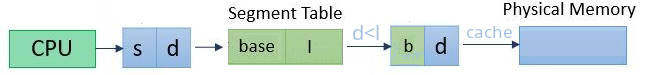
\includegraphics[scale=2.5]{./images/segmentation_01.jpeg}
  \end{figure}

\begin{enumerate}

  \item Segmentation
  \begin{enumerate}
    \item Logical address = segment number + offset
    \item Segment Table(ST) :
    \begin{enumerate}
      \item Base: starting address of the segment in memory.
      \item Limit(offset): It specifies the length of the segment.
      \item ST consumes less space
    \end{enumerate}
  \item User specifies the segment size, whereas, in paging, the hardware determines the page size.
  \item Segments can be shared.
  \item External fragmentation but no internal fragmentation.
  \item Compaction
  \end{enumerate}

  \item Paged Segmentation
  \item Segmented Paging
  \item Virtual memory
    \begin{enumerate}
    \item Swapping
    \item demand paging
    \item page replacement policies : FIFO, LRU, Optimal,
    \item Dirty bit, threshing
    \item Dynamic allocation policies, working set principle, window size
    \item Part of the process is in memory and the remaining is in secondary storage.
    \item Size of the program can be more than the memory size.
    \item Can be page based or segment based.
    \item OS allocates fixed frames to each process.
  \end{enumerate}

\end{enumerate}

% ----------------------------------------------------------------------------

% ----------------------------------------------------------------------------

% ----------------------------------------------------------------------------

% ----------------------------------------------------------------------------

% ----------------------------------------------------------------------------

% ----------------------------------------------------------------------------

% ----------------------------------------------------------------------------

% ----------------------------------------------------------------------------
